\documentclass[tikz,border=3.14mm]{standalone}
\usepackage{tikz}

\begin{document}
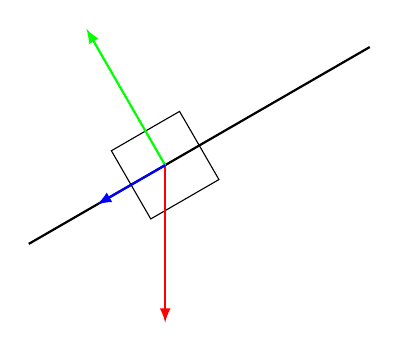
\begin{tikzpicture}

  % Define the angle of the inclined plane
  \def\angle{30}

  % Draw the inclined plane
  \draw[thick] (0,0) -- (\angle:5cm);

  % Draw the block
  \node[rectangle,draw,minimum size=1cm,transform shape,rotate=\angle] at (\angle:2cm) (block) {};

  % Draw the forces
  \draw[-latex,thick,red]  (block.center) -- +(270:2cm);   % gravity
  \draw[-latex,thick,green](block.center) -- +(\angle+90:2cm); % normal force
  \draw[-latex,thick,blue] (block.center) -- +(\angle-180:1cm); % friction

\end{tikzpicture}
\end{document}